\chapter{Origine Crétacéenne de la domestication virale chez les guêpes parasitoïdes Eucoilini}

Dans le chapitre précédent, la famille virale des Filamentoviridae a été présentée. Depuis les années 1970, des virus ayant une forme filamenteuse ont été identifiées chez plusieurs espèces de guêpes endoparasitoïdes. D'après nos travaux, ces virus font partie d'une nouvelle famille virale, les Filamentoviridae, et semblent adaptés de manière spécifique au mode de vie endoparasitoïde dont elles ont probablement exploité les particularités écologiques au cours de leur évolution. Le premier virus filamenteux à avoir été caractérisé au niveau moléculaire infecte le parasitoïde de \textit{Drosophile} \citep{lepetit_genome_2017}  \textit{Leptopilina boulardi}. Ce virus, surnommé Leptopilina boulardi filamentous virus (LbFV), a un effet sur le comportement de ponte des guêpes. En effet, contrairement aux femelles non infectées, les femelles infectées par ce virus acceptent de pondre leurs œufs chez des hôtes déjà parasités \citep{varaldi_infectious_2003,varaldi_artifical_2006}. Cette induction du "superparasitisme" permet la transmission horizontale du virus, augmentant ainsi la valeur adaptative du virus au détriment des guêpes \citep{gandon_superparasitism_2006}. De plus, ce virus est principalement transmis verticalement de la mère à la progéniture \citep{martinez_additional_2016}, ce qui a pu faciliter des échanges fortuits de matériel génétique entre le virus et les guêpes sur le long terme. Dans ce sens, des recherches récentes suggèrent que le génome entier d'un virus ancestral apparenté a été endogénisé chez l'ancêtre commun des guêpes appartenant au genre \textit{Leptopilina} (Di Giovanni et al., 2020). Aujourd'hui, 13 gènes filamenteux (EVEs) sont présents chez tous les individus de ce genre (Di Giovanni et al., 2020). Comme chez d'autres espèces de guêpes parasitoïdes qui ont domestiqué des virus  \citep{bezier_polydnaviruses_2009,volkoff_analysis_2010,pichon_recurrent_2015,burke_common_2019}, ces gènes filamenteux endogènes ont été domestiqués et sont utilisés par les guêpes femelles pour délivrer des facteurs de virulence, qui sont nécessaires pour protéger leurs œufs du système immunitaire de l'hôte \citep{colinet_convergent_2007,di_giovanni_behavior-manipulating_2020}. Plus précisément, dans ce système, une \textit{ADN polymérase} virale (ORF58) amplifie de manière temporaire une partie des EVEs (10/13) au moment où les VLPs sont formées. L'amplification génomique se traduit par une augmentation de la transcription de ces mêmes gènes. \\

Plusieurs de ces gènes amplifiés ont des rôles connus chez des virus "libres" : dans la transcription (\textit{lef-4}, \textit{lef-8} et \textit{lef-9}), dans l'enveloppement des protéines de virulence (\textit{ac81}) \citep{ dong_autographa_2016} et la formation de membranes lipidiques (\textit{lcat}) \citep{saeedi_review_2015}. Les "virus-like particles" (VLPs) sont des structures comparables à des liposomes. Elles sont en effet constituées d'une membrane lipidique contenant des facteurs de virulence sous la forme de protéines codées par les guêpes. Une fois entièrement assemblées, ces particules sont injectées avec l'œuf pendant l'oviposition et leur contenu est libéré au sein des cellules immunitaires de l'hôte, les hémocytes \citep{rizki_parasitoid_1990,colinet_convergent_2007}. Une fois à l'intérieur des cellules, les protéines de virulence génèrent des changements morphologiques importants qui empêchent les cellules d'initier une réponse immunitaire efficace contre l'œuf de parasitoïde \citep{colinet_convergent_2007}. En outre, nous savons que ces EVEs proviennent très probablement d'un seul événement d'endogénisation puisque les phylogénies des 13 EVEs sont identiques et congruentes avec celle des guêpes, et parce que nous détectons des conservations de blocs synténiques entre les génomes de guêpes. Cependant, aucune estimation de l'âge de cet évènement, ni de la diversité d'espèces concernée ne sont actuellement disponibles. Nous savons néanmoins que l'espèce éloignée du genre \textit{Ganaspis} ne présente aucune preuve d'endogénisation (Di Giovanni et al., 2020).\\

Afin d'étudier la diversité des guêpes impliquées dans cet évènement, nous avons donc recherché par PCR la présence de l'ORF le plus conservé (ORF96) chez 41 spécimens de Figitidae. En nous appuyant sur la phylogénie de \citep{blaimer_comprehensive_2020}, nous avons complété par l'analyse de trois espèces appartenant à cette tribu, \textit{Rhoptromeris}, \textit{Thrichoplasta}, \textit{Trybliographa}, et \textit{Leptolamina}, dont nous avons séquencé le génome.\\

Nous avons ensuite cherché de manière systématique des homologies de séquences avec tous les ORFs prédits de la famille des Filamentoviridae décrite au (\hyperref[sec:chap2]{chapitre 2}). À l'exception de l'espèce la plus basale du groupe "\textit{Leptolamina}", les six génomes d'Eucoilini présentaient des homologies de séquence élevées avec chacun des 13 EVEs signalés précédemment (\figurename{\ref{figure:Cynipoidea_EVE_heatmap_french}}). Les phylogénies de ces gènes (Type 1 sur la  \figurename{\ref{figure:Type_EVE_phylogenies_french}}) et la conservation de la synténie pour certains d'entre eux étaient cohérents avec un scénario d'endogénisation ancestrale chez l'ancêtre commun des 6 espèces d'Eucoilini. \\


\begin{figure}[!htpbt]
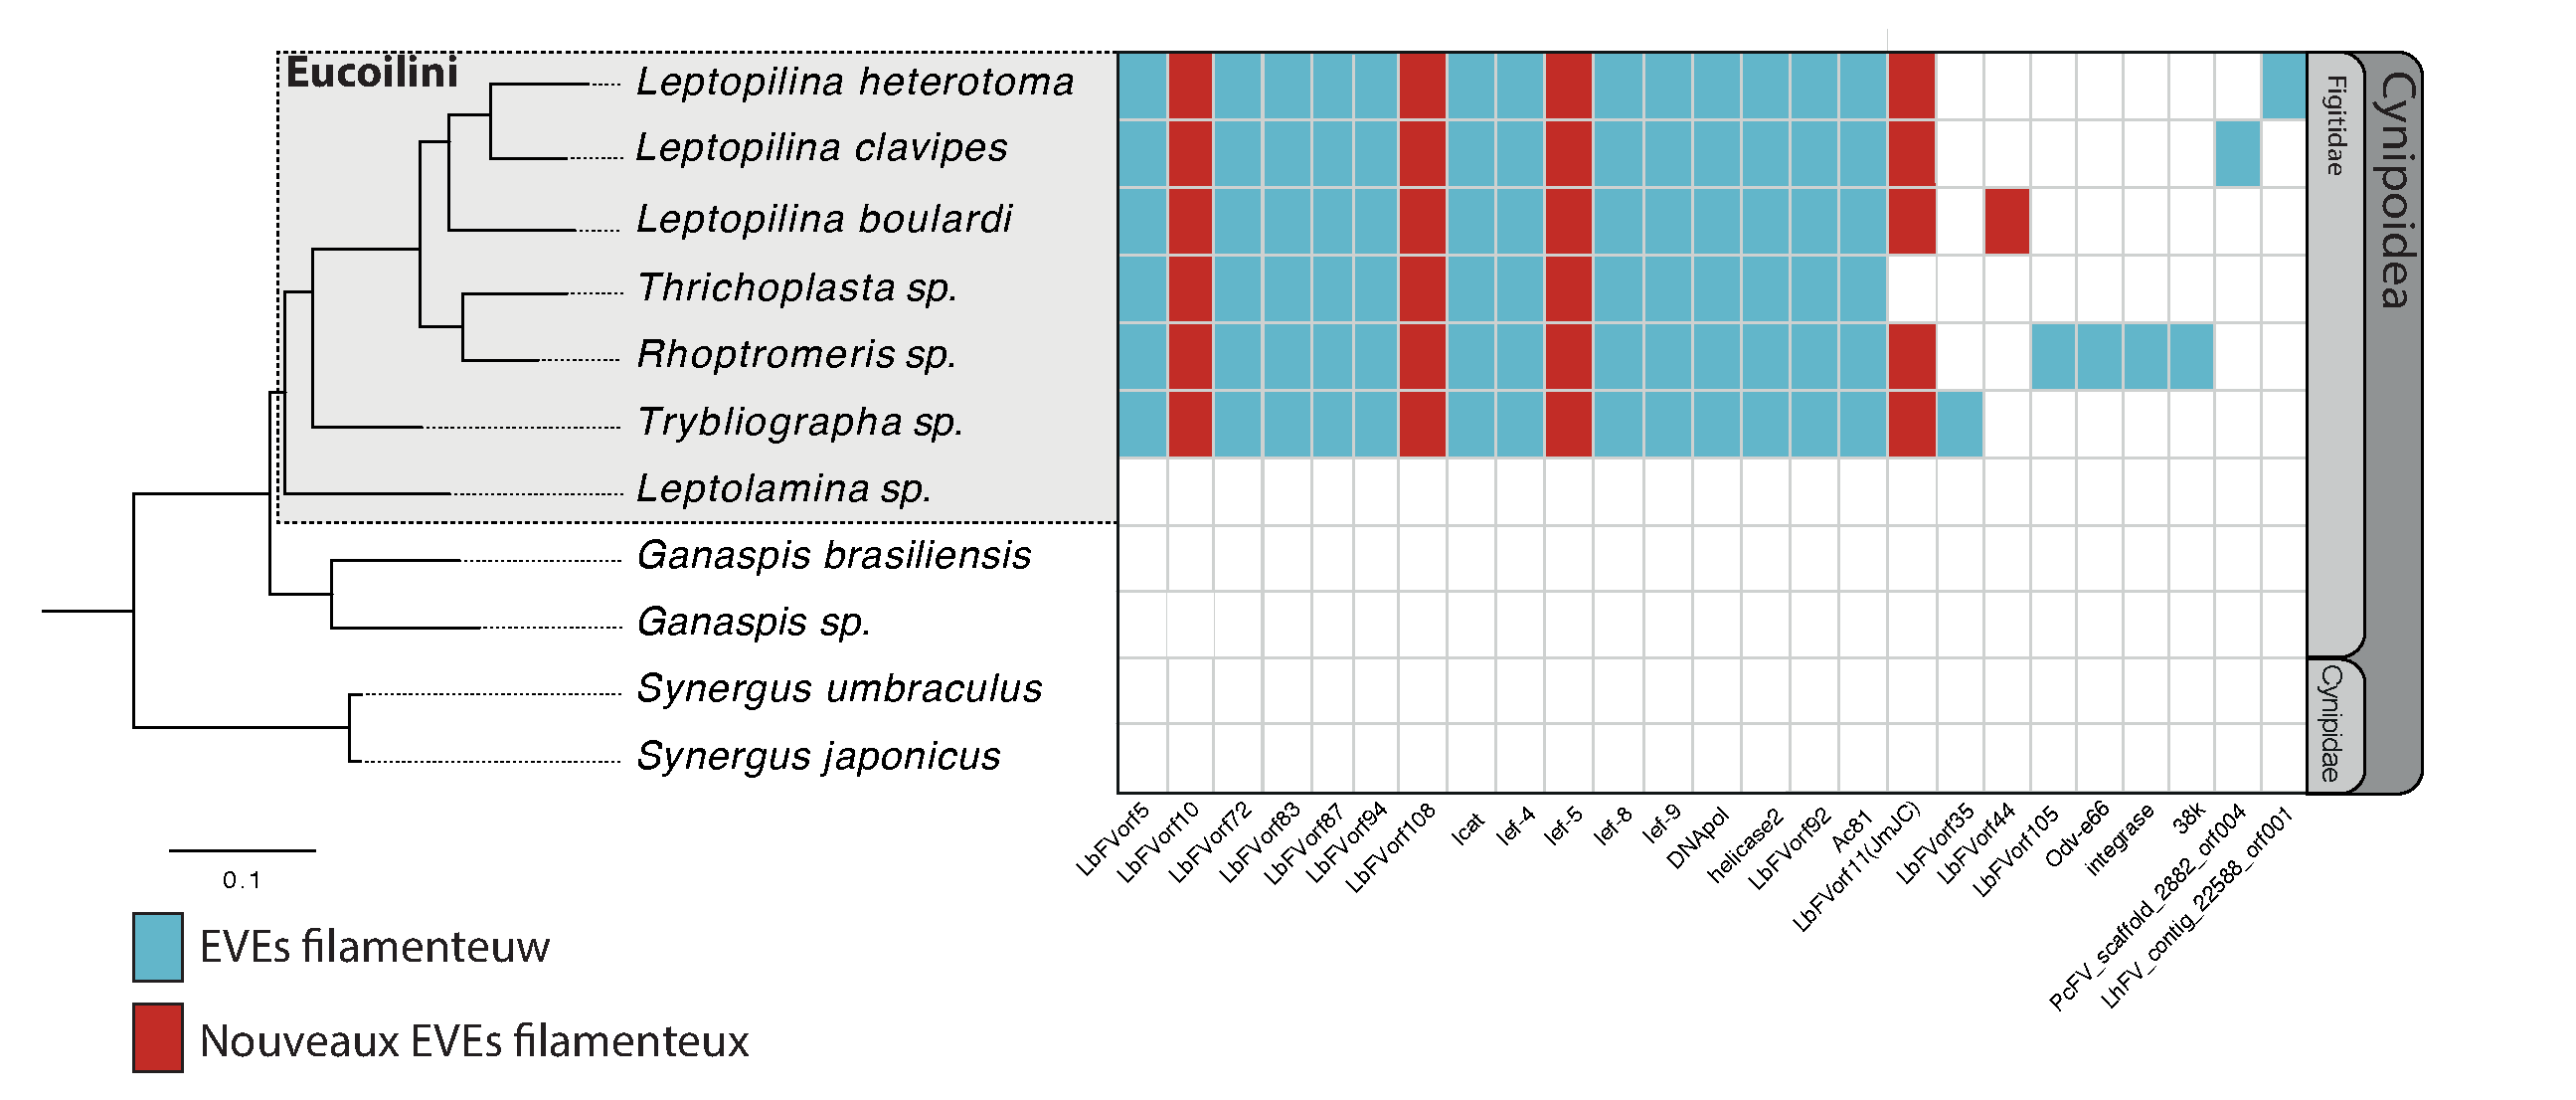
\includegraphics[width=\linewidth,height=\textheight,keepaspectratio]{PhD-master/figures/Cynipoidea_EVE_heatmap_french.pdf}\centering
\caption[Paper3:Distribution des EVE filamenteux parmi les espèces de Cynipoidea]{\textbf{Distribution des EVE filamenteux parmi les espèces de Cynipoidea}. La phylogénie des Cynipoidea a été estimée à l'aide de 1 000 gènes BUSCO. Chaque ligne représente une espèce de Cynipoidea, tandis que chaque colonne représente un EVE filamenteux.
Les cases bleues indiquent la présence d'EVE dans un génome, tandis que les cases blanches indiquent son absence. Les cases rouges indiquent les EVEs nouvellement assignés provenant du même évènement ancestral que dans \cite{di_giovanni_behavior-manipulating_2020}.}
\label{figure:Cynipoidea_EVE_heatmap_french}
\end{figure}


\begin{figure}[!htpbt]
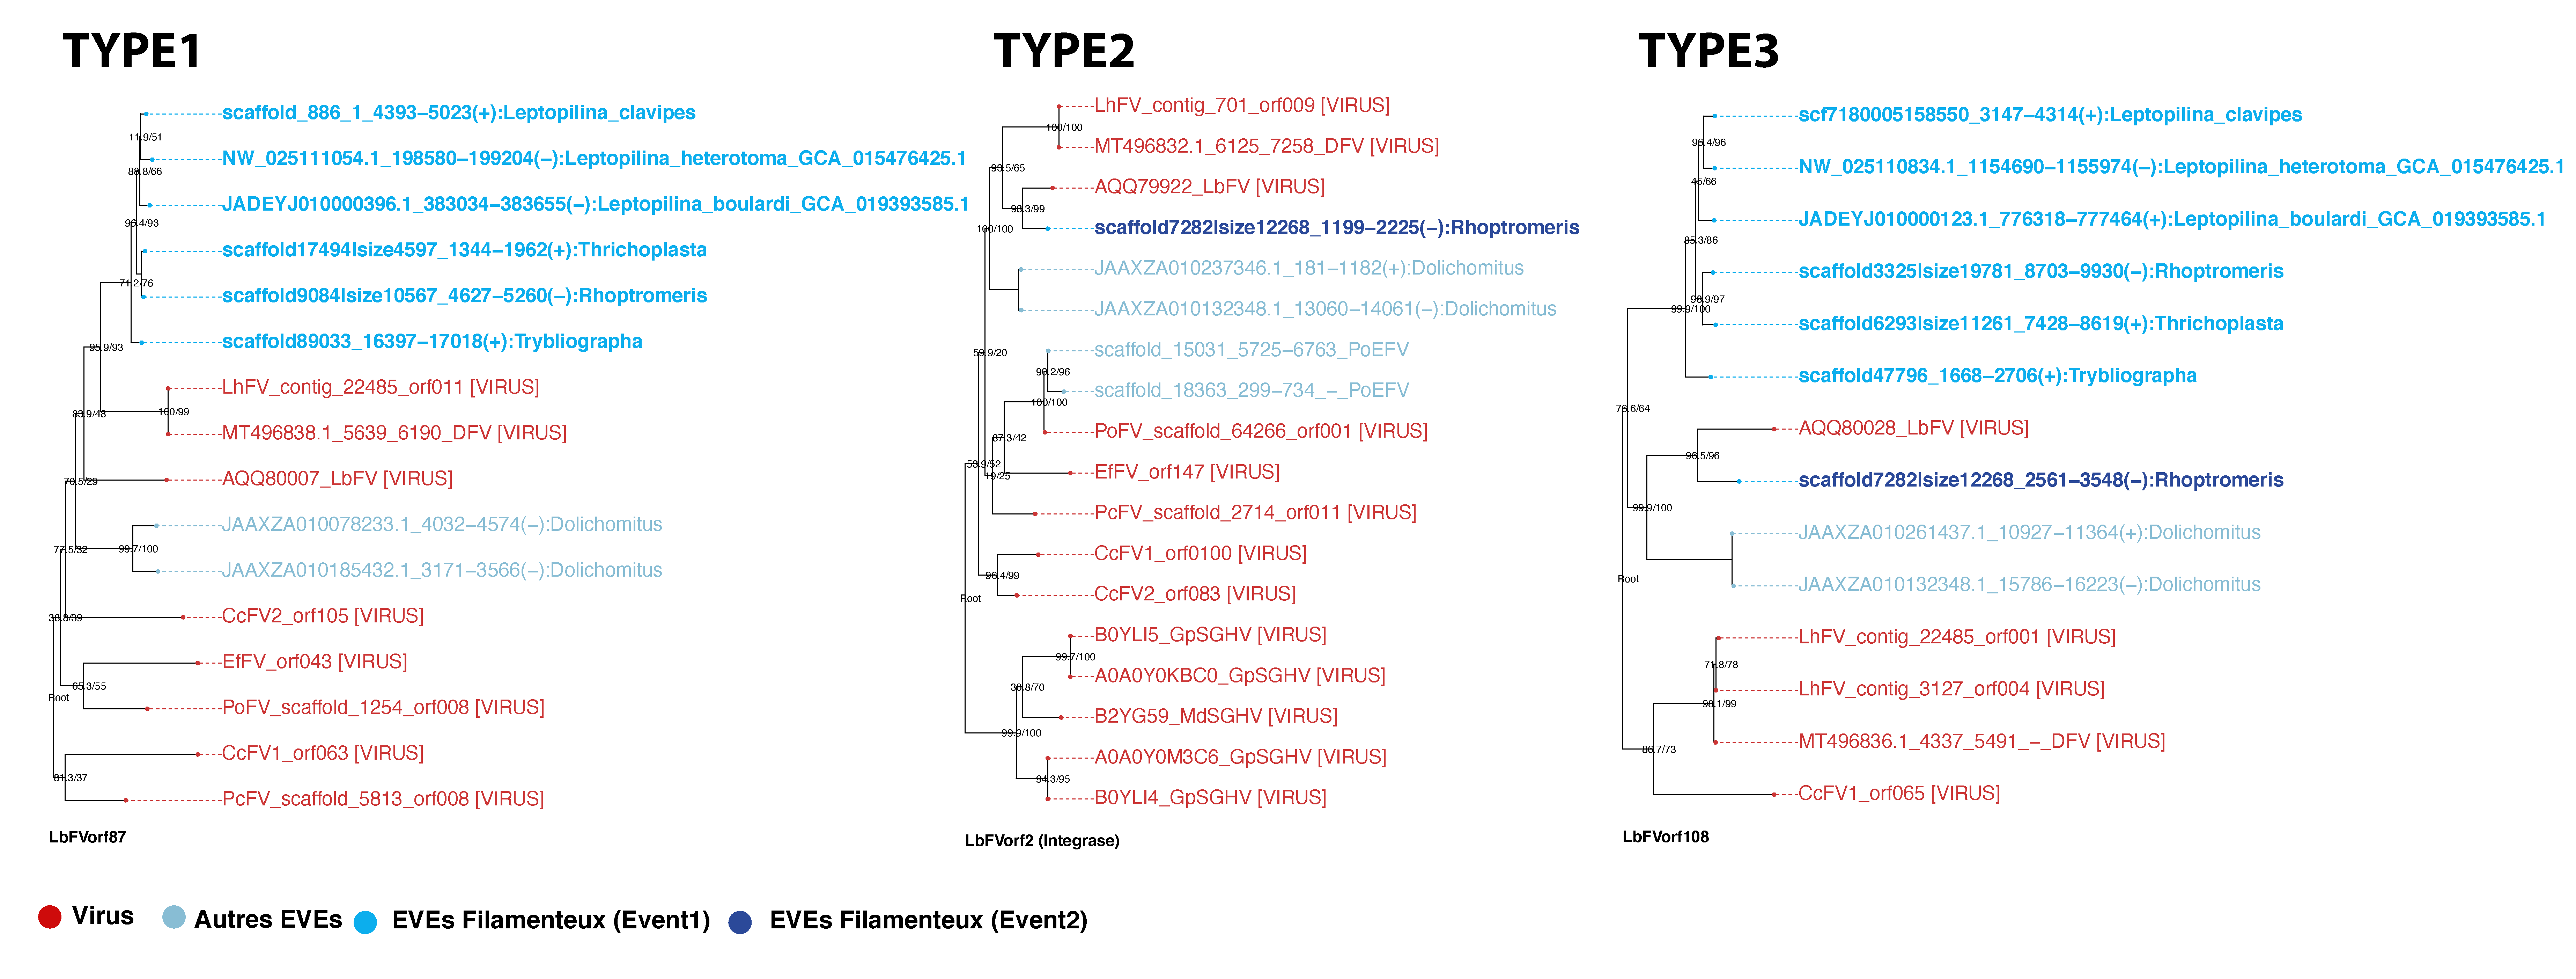
\includegraphics[width=\linewidth,height=\textheight,keepaspectratio]{PhD-master/figures/Type_EVE_phylogenies_french.pdf}\centering
\caption[Paper3:Type de phylogenies d'EVEs filamenteux chez les Eucoilini]{\textbf{Exemple de phylogénies d'EVEs filamenteux observées}. Le type1 correspond à un événement d'endogénisation unique qui s'est produit chez l'ancêtre de la majeure partie des Eucoilini et impliquant un donneur proche de LhFV. Le type2 suggère un autre événement indépendant qui s'est produit dans la branche \textit{Rhoptromeris} et impliquant un donneur proche de LbFV. Les phylogénies de type3 suggèrent que les deux événements se sont produits pour ce gène}.
\label{figure:Type_EVE_phylogenies_french}
\end{figure}

De plus, l'analyse a révélé la présence de 5 gènes supplémentaires (non identifiés par \cite{di_giovanni_behavior-manipulating_2020}) issus du même événement d'endogénisation. Comme attendu pour des gènes impliqués dans la formation de structures liées à la fitness des guêpes comme les VLPs, chacun de ces gènes présentait un régime de sélection purifiant. Bien que ces résultats indiquent que ces gènes sont étroitement associés à la fitness de ces guêpes, nous manquions de connaissances sur leurs conséquences phénotypiques  chez les espèces d'Eucoilini en dehors des \textit{Leptopilina}. Au cours de sa thèse de doctorat soutenue en 1999 à l'Université de Rennes, Nabila Kacem Haddj El Mrabet a décrit la présence de VLPs dans la glande à venin de \textit{Trybliographa rapae}(\figurename{\ref{figure:Microscopy_Lboulardi_Trybliographa_resume}}). Ces résultats, obtenus sur l'espèce la plus basale du groupe concerné par l'évènement d'endogénisation, permettent d'envisager que l'ensemble des espèces, depuis les \textit{Leptopilina} et jusqu'aux \textit{Trybliographa}, produisent effectivement des VLPs grâce aux gènes filamenteux domestiqués.\\

\begin{figure}[H]
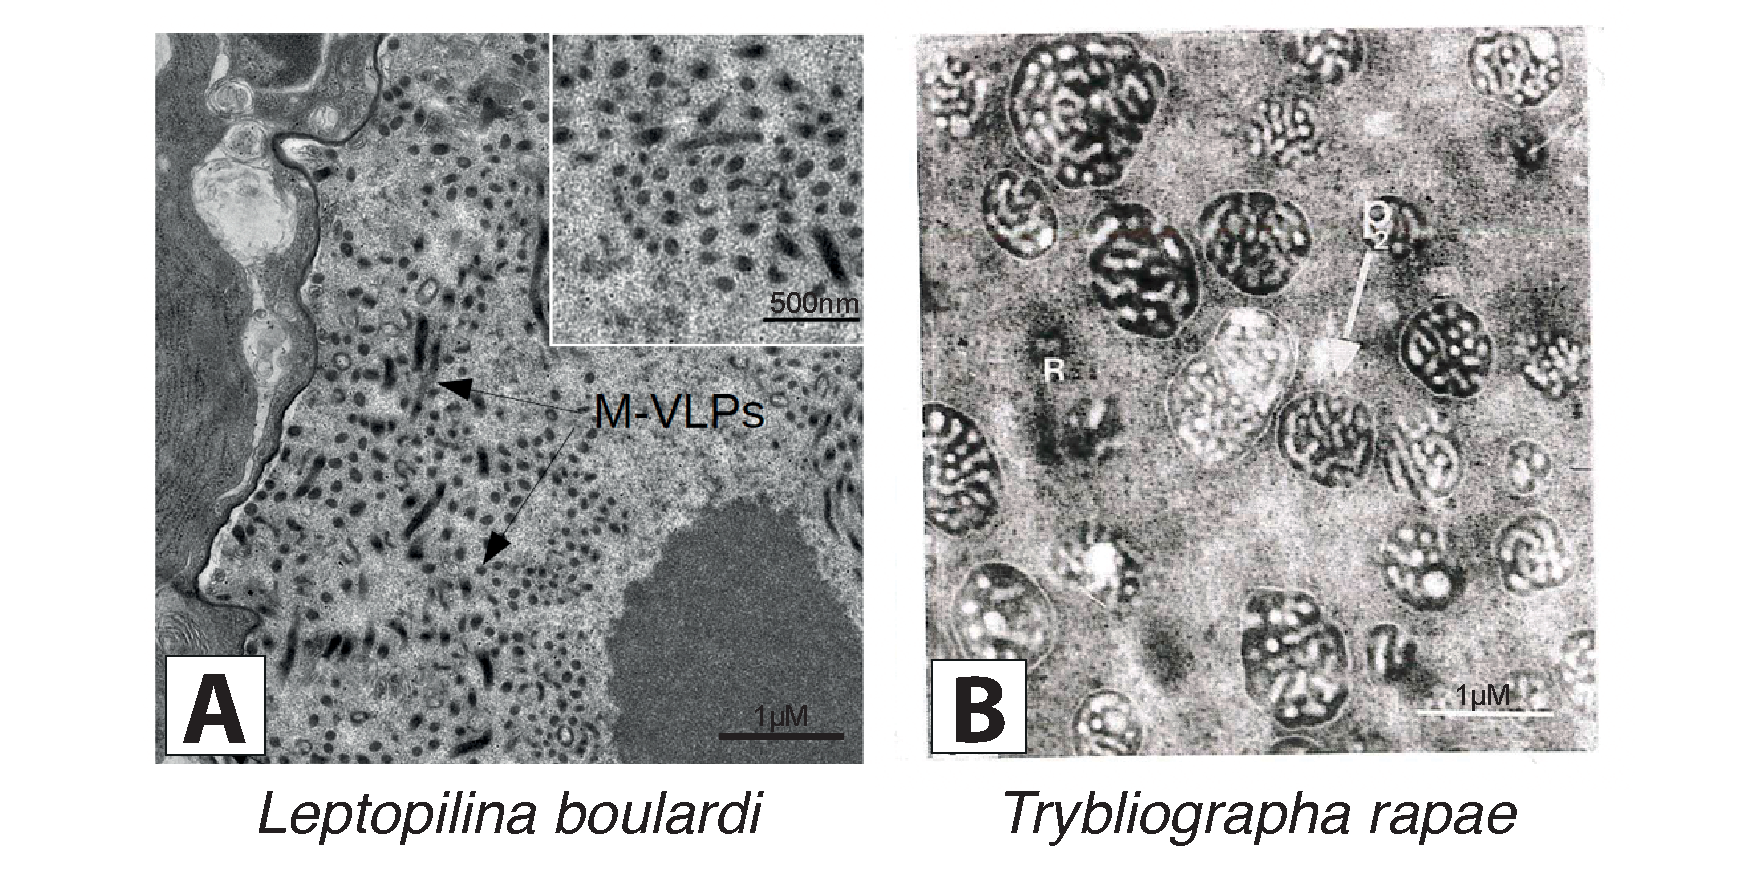
\includegraphics[width=\linewidth,height=\textheight,keepaspectratio]{PhD-master/figures/Microscopy_Lboulardi_Trybliographa_resume.pdf}\centering
\caption[Paper3:[Microscopie électronique des VLPs chez \textit{L.boulardi} et \textit{T.rapae}]{Photos de microscopies électroniques des VLPs produits dans la glande à venin de \textit{Lepoptilina boulardi} (A) et \textit{Trybliographa rapae} (B) provenant respectivement de \cite{di_giovanni_behavior-manipulating_2020} et D.Poinçot et K.Haddj E PhD 1999.}
\label{figure:Microscopy_Lboulardi_Trybliographa_resume}
\end{figure}

En plus de cet évènement majeur d'endogénisation virale, nous avons également découvert une endogénisation plus récente chez \textit{Rhoptromeris}. Cet événement implique 9 EVEs, dont certains sont pseudogénisés et d'autres sont encore intacts et dont les phylogénies représentent des topologies de type 2 et 3 (\figurename{\ref{figure:Type_EVE_phylogenies_french}}). De façon remarquable, l'un des 18 gènes identifiés dans l'événement initial semble avoir été remplacé par un gène homologue provenant de ce deuxième événement chez \textit{Rhoptromeris}. \\

Nous avons observé des similitudes structurelles entre ce gène et une protéine de Hantavirus qui remplit une fonction impliquée dans les mécanismes d'entrée virale dans les cellules hôtes \citep{guardado-calvo_surface_2021}. Le remplacement de ce gène chez cette espèce pourrait avoir amélioré l'efficacité avec laquelle les VLPs produits par \textit{Rhoptromeris} pénètrent dans les cellules immunitaires de leurs hôtes Diptères de la famille des Chloropidae.\\

Pris dans leur ensemble, ces résultats indiquent qu'un événement d'endogénisation s'est donc produit chez l'ancêtre commun de ces 6 espèces d'Eucoilini, il y a environ 75 millions d'années, selon une estimation récente de l'age de ce nœud dans la phylogénie des Cynipoidea \citep{blaimer_comprehensive_2020}. La période estimée de cet événement coïncide avec la diversification des Diptères Schizophora qui sont les hôtes de ces guêpes parasitoïdes \citep{wiegmann_episodic_2011} (\figurename{\ref{figure:Schizophora_Eucoilini_virus_phylogeny_french}}). Nous pouvons donc émettre l'hypothèse que la production de VLPs, aurait permis à ces espèces de coloniser et de s'adapter à de nombreux hôtes Schizophora au cours de la radiation du groupe. \\

\begin{figure}[!htpbt]
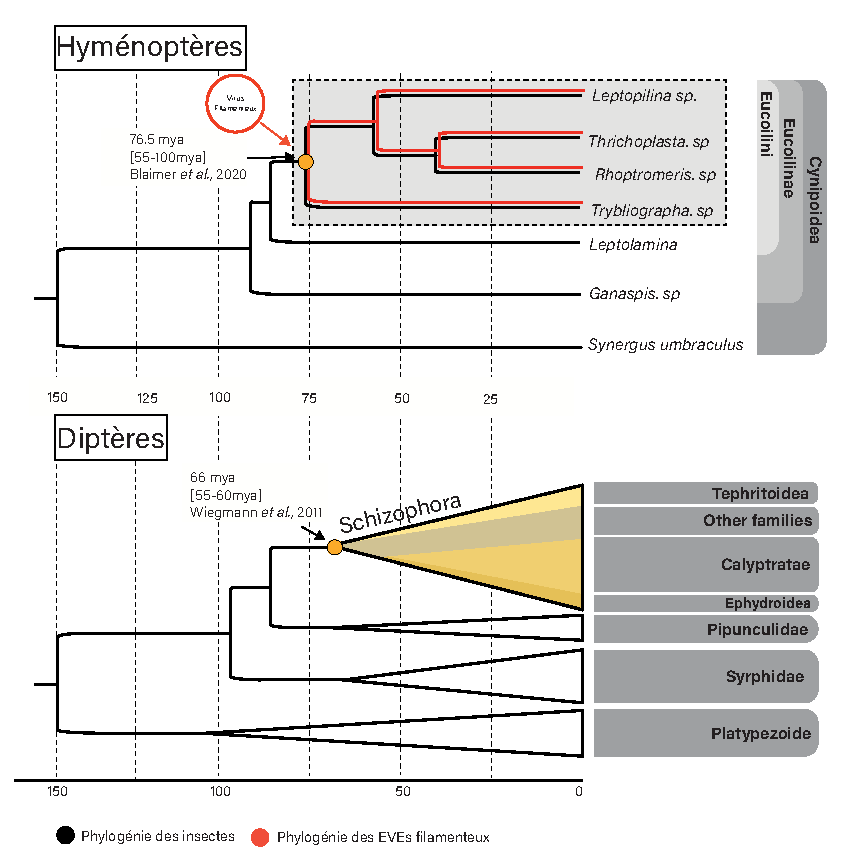
\includegraphics[width=\linewidth,height=\textheight,keepaspectratio]{PhD-master/figures/Schizophora_cynipids_virus_phylogeny_french.pdf}\centering
\caption[Paper3:Arbres phylogénétiques des Eucoilini et des EVEs filamenteux]{\textbf{Arbres phylogénétiques des hôtes et des EVEs filamenteux}. Les branches noires correspondent aux branches des Hyménoptères (en haut) ou des Diptères (en bas), tandis que les branches rouges correspondent aux branches des EVEs filamenteux. Les arbres ont été reconstruits en utilisant les sources suivantes :\citep{blaimer_comprehensive_2020} pour les données sur les Hyménoptères, et \citep{wiegmann_episodic_2011} pour la phylogénie des Diptères. La phylogénie des virus filamenteux endogènes a été déduite de la concaténation des 16 éléments viraux filamenteux endogènes partagés par tous les Eucoilini).}
\label{figure:Schizophora_Eucoilini_virus_phylogeny_french}
\end{figure}

\newpage
Enfin, en utilisant les données fournies par l'événement d'endogénisation chez les Eucoilini (impliquant un virus filamenteux permettant la formation de VLPs) et celui impliquant les guêpes du complexe des Microgastroïde (impliquant un nudivirus et permettant la production de  polydnavirus), nous avons pu calibrer la phylogénie des \textit{Naldaviricetes}, à laquelle appartiennent les deux virus donneurs. Les inférences estiment que les Filamentoviridae seraient apparus il y a 250 à 350 millions d'années, ce qui coïncide avec le moment où les Hyménoptères ont commencé à se diversifier entre le Carbonifère et le Trias (239-329 millions d'années) \citep{peters_evolutionary_2017}. Les Filamentoviridae sont des virus qui semblent être spécifiques des Hyménoptères, et selon toute vraisemblance plus spécifiquement aux guêpes endoparasitoïdes. Plus spécifiquement, les lignées de guêpes parasitoïdes les plus diverses (c'est-à-dire Ceraphronoidea, Ichneumonoidea et Proctotrupomorpha) ont connu une extraordinaire radiation entre 195 et 265 millions d'années \citep{peters_evolutionary_2017}. Par conséquent, nous pourrions spéculer que ces virus seraient apparus au moment de la diversification des Hyménoptères avant de se specialiser sur les lignées de guêpes endoparasitoïdes. La longue histoire évolutive commune a ensuite entrainé l'endogénisation accidentelles de virus dans un processus dynamique, comme nous avons pu l'observer chez  \textit{Rhoptromeris}. Néanmoins, ces données montrent qu'il est difficile de remplacer une machinerie virale complète si les gènes nouvellement acquis ont des fonctions redondantes au système déjà en place, mais concernerait plutôt le remplacement de quelques gènes dans un système déjà établi.  Le seul exemple supplémentaire de remplacement d'une machinerie virale entière serait chez \textit{V. canescens}, où un ichnovirus (polydnavirus) aurait été remplacé par un nudivirus (VLPs) \citep{pichon_recurrent_2015}. Cependant, l'analyse faite dans le (\hyperref[sec:chap1]{chapitre 1}) (qui incluait \textit{V. canescens}), n'a pas permis de confirmer ce remplacement.\\

Ces travaux complets en anglais sont disponibles dans la troisième section du chapitre \hyperref[sec:chap3]{Études}. 


